
\section{TikZ Styles}

The following shows the different line widths you can use when drawing in TikZ. This should be an optional argument to the draw command.


\begin{figure}[H]
\centering
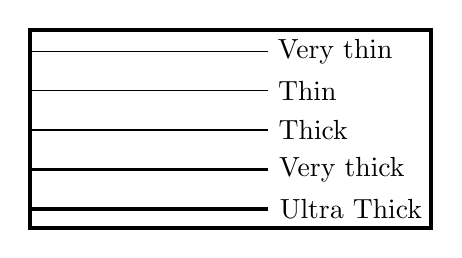
\begin{tikzpicture}[yscale=0.5]
\draw[very thin] (0,0) -- (3,0) node[right] {Very thin};
\draw[thin] (0,-1) -- (3,-1) node[right]{Thin};
\draw[thick] (0,-2) -- (3,-2) node[right]{Thick};
\draw[very thick] (0,-3) -- (3,-3) node[right]{Very thick};
\draw[ultra thick] (0,-4) -- (3,-4) node[right]{Ultra Thick};

\draw[ultra thick] (current bounding box.north east) rectangle (current bounding box.south west);

\end{tikzpicture}
\caption{Line Widths}
\end{figure}

%------------------

\begin{figure}[H]
\centering
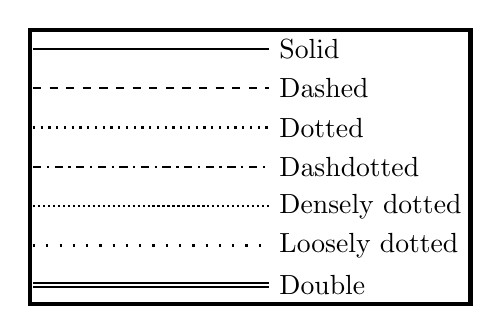
\begin{tikzpicture}[yscale=0.5]

\draw[thick,solid] (0,0) -- (3,0) node[right]{Solid};

\draw[thick,dashed] (0,-1) -- (3,-1) node[right]{Dashed};

\draw[thick,dotted] (0,-2) -- (3,-2) node[right]{Dotted};

\draw[thick,dashdotted] (0,-3) -- (3,-3) node[right] {Dashdotted};

\draw[thick,densely dotted] (0,-4) -- (3,-4) node[right] {Densely dotted};

\draw[thick,loosely dotted] (0,-5) -- (3,-5) node[right] {Loosely dotted};

\draw[thick,double] (0,-6) -- (3,-6) node[right] {Double};

\draw[ultra thick] (current bounding box.north east) rectangle (current bounding box.south west);
\end{tikzpicture}
\caption{Line Styles}
\end{figure}

%------------------
\begin{figure}[H]
\centering
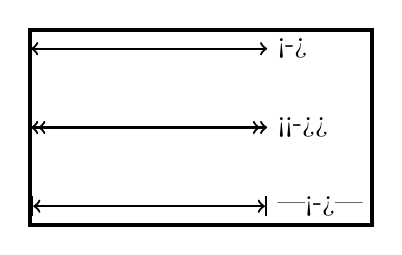
\begin{tikzpicture}[thick]
\draw[<->] (0,0) -- (3,0) node[right]{\lstinline{<->}};

\draw[<<->>] (0,-1) -- (3,-1) node[right]{\lstinline{<<->>}};

\draw[|<->|] (0,-2) -- (3,-2) node[right]{\lstinline{|<->|}};

%\draw[-*] (0,-3) -- (3,-3) node[right]{\lstinline{-*}};

\draw[ultra thick] (current bounding box.north east) rectangle (current bounding box.south west);
\end{tikzpicture}
\caption{Arrow Head Types}
\end{figure}



%------------------
\begin{figure}[H]
\centering
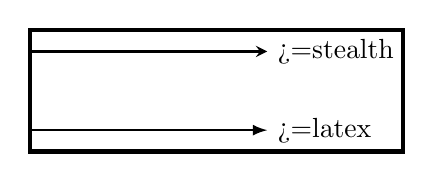
\begin{tikzpicture}[thick]

\draw[->,>=stealth] (0,0) -- (3,0) node[right]{\lstinline{>=stealth}};

\draw[->,>=latex] (0,-1) -- (3,-1) node[right]{\lstinline{>=latex}};


\draw[ultra thick] (current bounding box.north east) rectangle (current bounding box.south west);
\end{tikzpicture}
\caption{Arrow Header Styles}
\end{figure}


%% Rotational Circular Geometry

Figure \ref{Fig:rotationalcirculargeometry} shows rotational circular geometry typically seen in \textit{Dynamics}, drawn in TikZ.

\begin{figure}[H]
\centering
\begin{tikzpicture}[xscale=0.8,yscale=0.8]
% draw circle
\shadedraw[inner color=gray!10,outer color=gray!40, draw=black, very thick] (0,0) circle (3cm);

\tikzmath{
	\y = -45 + 90;
	\z = 90 - 45;
}

\draw[guide] (0,0) -- (\y:4cm);
\draw[guide] (0,0) -- (-45:5cm);
\draw[guide] (0,0) -- (5,0);

% phi-theta
\draw[->, very thick, blue] (5,0) arc (0:\z:5cm) node[label] {$\phi-\theta(t)$};

% phi
\draw [<-, very thick, space] (\y:4cm) arc (\y:-45:4cm) node[label] {$\phi$};

% theta
\draw[->, very thick] (5, 0) arc (0:-45:5cm) node[label] {$\theta(t)$};

% base vectors
%\draw[basevec] (\z:4cm) -- (\z:5cm);
%\draw[basevec] (\z:4cm) -- +(\z+90:1cm);
\nandm{45:4cm}{45}

% Points of interest
\poi{0,0}
\poi{-45:4cm}
\poi{5,0}

\end{tikzpicture}
\caption{Rotational Circular Geometry}
\label{Fig:rotationalcirculargeometry}
\end{figure}